Homologno križanje \cite{crxSizeFair} temelji se na prirodnom svojstvu križanja, homologiji. Homologija u prirodi osigurava da se križanje uvijek događa između organizama koji imaju uglavnom identične sekvence gena unutar kromosoma. Ovime se podupire nedestruktivno križanje - kombiniraju se geni koji rade točno određenu ulogu, gdje je uloga uvjetovana pozicijom samog gena.

Homologno križanje, u smislu križanja u genetskom programiranju, koristi pozicijsku homologiju. Pozicijska homologija potiče izmjenu genetskog materijala samo ako se ono događa na istoj, ili dovoljno bliskoj poziciji unutar dva genoma.

Uobičajeni operatori križanja, prilikom odabira podstabala ili čvorova koji sudjeluju u križanju uglavnom ne uzimaju u obzir njihovu poziciju. Ne uzimajući to u obzir, nerijetko dolazi do naglog rasta jedinki svakom novom generacijom (\textit{eng. bloat}). Budući da ovi operatori najčešće ne uzimaju u obzir prekomjeran rast jedinki koje proizvode, potrebno je modificirati sam algoritam tako da se prevelike jedinke kažnjavaju manjom dobrotom. Time, iako možda novonastala jedinka izvrsno rješava zadan problem, može se dogoditi da bude odbačena zbog svoje veličine. Iz razloga što se ne uzimaju u obzir pozicije niti veličine podstabala koja sudjeluju u križanju, mala je šansa da će novonastala jedinka biti u okviru željene veličine, povećavajući šansu da će u budućnosti zbog te veličine i izumrijeti. Drugi razlog zbog kojega prekomjeran rast jedinke nije dobar, a usko je povezan s prethodnim, je taj da, u prevelikoj jedinci vjerojatno postoji puno nepotrebnog ponašanja - ponašanje koje nije potrebno, a kroz generacije je preživjelo samo zato što ne donosi nikakvu štetu.

Drugi problem koji se javlja kod uobičajenih operatora križanja je taj da ti operatori potpuno nasumično prenose dijelove programa u novu jedinku. Budući da je taj fragment jedinke preživio proces selekcije, za pretpostaviti je da postoji velika šansa da on predstavlja relevantan dio za put do konačnog rješenja. Također, velika je šansa da korisnost istog fragmenta uvelike ovisi i o kontekstu u kojem se on izvršava. Stavljajući takav fragment na nasumično mjesto u novu jedinku donosi šansu da će taj kontekst biti uništen.

Kako bi se ovi problemi riješili prilikom samog križanja, a time se i povećale šanse za kvalitetu i nastavak života potomaka, homologni operator križanja prilikom samog križanja uzima u obzir i veličinu i poziciju podstabala roditelja koja će se iskrižati. Ovime se u samoj srži operatora sprječava prekomjeran rast potomaka i s većom vjerojatnošću nego inače, podržava prijenos konteksta pojedinih fragmenata rješenja u ono novonastalo.

Ovo križanje u stvari je inačica križanja pravednog s obzirom na veličinu. Odabir potencijalnih podstabala drugog roditelja potpuno je jednak u ovom križanju kao i kod križanja pravednog s obzirom na veličinu. Razlika u tome je ta da se, između svih potencijalnih podstabala drugog roditelja koji bi mogli sudjelovati u križanju, odabire ono podstablo koje je najbliže točki prekida prvog roditelja. Na slici \ref{crxHomo} prikazan je jedan takav primjer križanja - od dva potencijalna podstabala drugog roditelja, za križanje je odabrano ono koje je bliže točki prekida u prvom roditelju.

\begin{figure}[H]
	\centering
	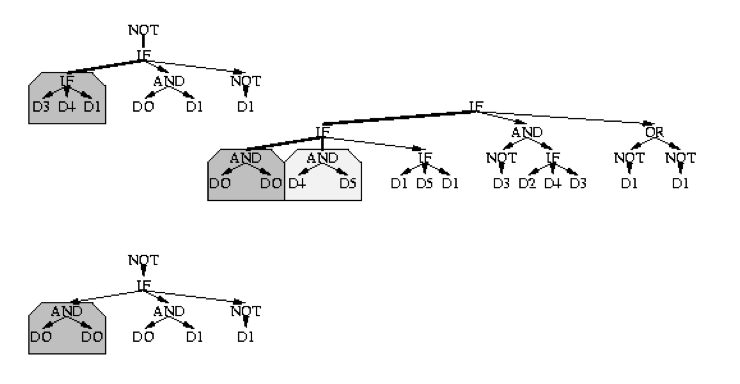
\includegraphics[scale=0.6]{./slike/crxHomo.png}
	\caption{Primjer homolognog križanja}
	\label{crxHomo}
\end{figure}

\subsection{Dosadašnji rezultati}
U \cite{crxSizeFair}  provedeno je istraživanje nad četiri različita problema; po dva za simboličku regresiju (polinomi petog i šestog stupnja) i po dva za logičke funkcije (6 i 11 - multipleksor). Pokazano je kako homologno križanje po sposobnosti pronalaska rješenja danih problema nije značajno bolje od križanja pravednog s obzirom na veličinu. No, kao i kod križanja pravednog s obzirom na veličinu, pokazano je kako je ovo križanje vrlo učinkovito prilikom sprječavanja pojave prekomjernog rasta jedinki.

Razlog sličnosti u rezultatima s križanjem pravednim s obzirom na veličini može biti prouzrokovano različitim razlozima. Jedan od razloga je mogućnost da kod ovog operatora u nekim slučajevima nije postojao izbor podstabla koji bi bio u skladu s homologijom, te bi operator bio primoran odabrati podstablo koje ne odgovara u potpunosti načelu odabira. Postojanje ovog slučaja pokazano je u spomenutom radu.

